\clearpage
\section{Tiny Garble}

\begin{refsection}

\begin{tcolorbox}	
\begin{tabular}{p{2.75cm} p{0.2cm} p{10.5cm}} 	
\textbf{Students Name}      &:& Goncalo Vitor (15/06/2018 - )\\
\textbf{Goal}               &:& Implementation of secure multy-party computation based on the Tiny Garble framework.\\
\textbf{Directory}          &:& \\
\end{tabular}
\end{tcolorbox}

This subsection will cover the installation and usage of TinyGarble, a GC framework that allows two parties to safely compute any function with their private inputs through Yao's Garbled Circuit Potocol. It accepts HDL and C/C++ as user inputs, although HDL will be the primary focus.

\subsection{Installation}

Since TinyGarble and most of the tools mentioned below have been mostly tested on Linux, it will be assumed that the user is running Linux on a virtual machine (VM), or directly from a partition. To do the former one can use Oracle's VirtualBox, which can be downloaded at \url{https://www.virtualbox.org/wiki/Downloads}. A copy of Linux is also needed, for this section Ubuntu 18.04 was used, found at \url{https://www.ubuntu.com/download/desktop}.

After installing and opening VirtualBox, select 'New', a Window should pop up asking for a name for the new VM, it doesn't matter, and for type and version, which should be Linux and Ubuntu respectively. The next step is choosing the amount of RAM that is going to be dedicated to the VM,  it depends on the system, but anything between 2048 and 4096 MB should be fine, 1024 MB or lower if the host PC has small amount of memory. Next create a virtual hard disk of VDI type, and choose dynamic or fixed size disk, it comes down to user preference. For the size of the disk, 10GB was enough to install and use TinyGarble properly, but slightly more is advisable.
After creating the virtual machine, it should ask for a start-up disk when launching it for the first time, select the Linux ISO file that was downloaded before. After that the installation of linux is pretty straight forward.

For TinyGarble to work, some dependencies have to be installed first, on Ubuntu it can be done with the following lines:

\begin{lstlisting}[caption={Installation of TinyGarble's dependencies}, language=bash, captionpos=b]
$ sudo apt install git
$ sudo apt install build-essential
$ sudo apt install libssl1.0-dev
$ sudo apt install libboost-all-dev
$ sudo apt install cmake
\end{lstlisting}

After this step i'ts necessary to clone TinyGarble's repository, at \url{https://github.com/esonghori/TinyGarble}, and build it. For this section it was cloned at the home directory '~'.

\begin{lstlisting}[caption={Configuration and compilation of TinyGarble. 'Sudo ./configure' and 'sudo make' may be needed.}, language=bash, captionpos=b]
$ git clone https://github.com/esonghori/TinyGarble.git
$ cd TinyGarble/
$ ./configure
$ cd bin/
$ make
\end{lstlisting}

To be able to use TinyGarble, a RTL Synthesis tool is also needed, to translate Verilog files into Netlist ones. In the example showed later, Yosys-abc is used. Which can be installed on Ubuntu 15.04 or higher with:

\begin{lstlisting}[caption={Installation of Yosys-abc for Ubuntu 15.04>}, language=bash, captionpos=b]
$ sudo apt-get install yosys
\end{lstlisting}

If on Ubuntu 14.04 or lower, a repository needs to be added first:

\begin{lstlisting}[caption={Installation of Yosys-abc for Ubuntu 14.04<}, language=bash, captionpos=b]
$ sudo add-apt-repository ppa:saltmakrell/ppa
$ sudo apt update
$ sudo apt install yosys
\end{lstlisting}

\newpage

\subsection{Usage}

\begin{figure}[H]
	\centering
	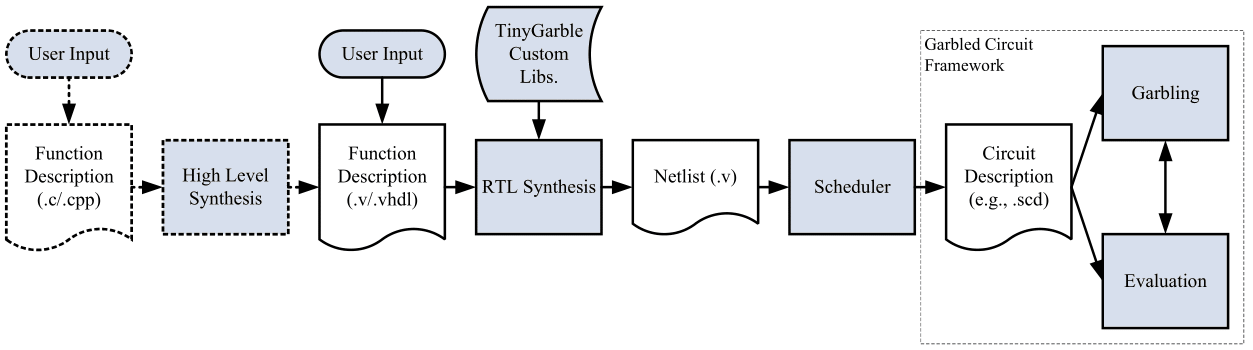
\includegraphics[width=1\textwidth, height=3cm]{./sdf/tiny_garble/figures/tiny_garble_flow.png}
    \caption{TinyGarble Global Flow\cite{Songhori}}\label{fig:tinygarble_flow}
\end{figure}

Following TinyGarble's global flow showed on the image above, it's possible to see that a C/C++ or Hardware Design Language (HDL) input is necessary. The former is slightly worse in terms of performance, since it needs an extra step of synthesis, with the help of a High Level Synthesis (HLS) tool, like Spart or Xilinx Vivado for C, to compile the C/C++ file into HDL, causing the end SCD file to have more logical gates than when using HDL input directly. This section mostly covers Verilog, since it's the most direct input, if VHDL input is needed, check the subsection UsingVHDL.

When writting the input file, some attention to the circuit's ports is needed, since TinyGarble's V2SCD (Netlist Verilog to SCD converter) accepts netlist files with a special format.
Below are the ports that can be used and what they represent.

\begin{itemize}
\item clk: clock cycle
\item rst: active high reset
\item g\_init: garbler's initial values, it's read only at the first clock, so it has to be saved on some register at the first rising edge
\item e\_init: evaluator's initial values, same as above
\item g\_input: garbler's input, it's read at every clock, so if the input was defined at N bits, and the circuit is executed X times, the total size of the input will be N * X bits, and each clock will shift the g\_input to the left N bits;
\item e\_input: evaluator's input, same as above
\item o: output, same as above, but TinyGarble executable has the option to show all the outputs of each clock concatenated, separated, or only show the last clock output
\end{itemize}

\newpage

Below it's an example of an and\_gate written in verilog with the format above.

\begin{lstlisting}[caption={and\_gate.v}, language=Verilog, captionpos=b]
module and_gate (input g_input, e_input, output o);
	assign o = g_input & e_input;
endmodule
\end{lstlisting}

Using TinyGarble's custom library, asic\_cell\_yosys\_extended.lib", located at TinyGarble/ciruit\_synthesis/lib/, and assuming that the Verilog file is in a folder named "circuits" located at the home directory '~', the compilation for the circuit can be done with the following instructions:

\begin{lstlisting}[caption={Yosys instructions to compile the combinational circuit Verilog file into a Netlist File. 'Sudo yosys' may be needed.}, language=bash, captionpos=b]
host@ubuntu:~$ yosys
yosys> read_verilog TinyGarble/circuit_synthesis/syn_lib/*.v
yosys> read_verilog circuits/and_gate.v 
yosys> hierarchy -check -top and_gate
yosys> proc; fsm; flatten; opt;
yosys> techmap; opt; 
yosys> dfflibmap 
-liberty TinyGarble/circuit_synthesis/lib/asic_cell_yosys_extended.lib
yosys> abc 
-liberty TinyGarble/circuit_synthesis/lib/asic_cell_yosys_extended.lib 
-script TinyGarble/circuit_synthesis/lib/script.abc; 
yosys> opt; clean; 
yosys> opt_clean -purge
yosys> stat
-liberty TinyGarble/circuit_synthesis/lib/asic_cell_yosys_extended.lib
yosys> write_verilog -noattr -noexpr sum_syn_yos.v				
\end{lstlisting}

The first 'read\_verilog' command is optional, it loads some circuits described in Verilog modules, to see which modules are available check 'TinyGarble/circuit\_synthesis/syn\_lib'. For this case in particular no exterior module was needed, so the command won't really do anything.
The 'stat' command is only used to show statistics of the final circuit configuration, optional as well.
These instructions should work for any combinational or sequential circuit.

The inscructions can be saved in a file ending with '.yos', and be used as a script in yosys, as the following shows:
\begin{lstlisting}[caption={Running yosys instructions contained in a script file.}, language=bash, captionpos=b]
host@ubuntu:~$ yosys
yosys> script file.yos
\end{lstlisting}

\newpage

Following the instructions the Netlist file below should be generated.

\begin{lstlisting}[caption={and\_gate\_netlist.v}, language=Verilog, captionpos=b]
module and_gate( g_input,  e_input, o);
  input g_input;
  input e_input;
  output o;
  AND _0_ (
    .A(e_input),
    .B(g_input),
    .Z(o)
  );
endmodule
\end{lstlisting}

The Netlist file can then be converted into a SCD file with the instruction below:

\begin{lstlisting}[caption={Installation of Yosys-abc}, language=bash, captionpos=b]
host@ubuntu~$ ./TinyGarble/bin/scd/V2SCD_Main 
-i circuits/and_gate_netlist.v-o circuits/and_gate.scd		
\end{lstlisting}

Before executing the SCD file, it can be tested with TinyGarble's SCD\_Evaluator\_Main located at TinyGarble/bin/scd. The '-c' option is the number of cycles, and the output\_mode differs the way the output is shown, 0 for concatenated(from all clocks), 1 for separated(for each clock), and 2 to show only the last clock output.

\begin{lstlisting}[caption={Testing a SCD file}, language=bash, captionpos=b]
host@ubuntu~$ ./TinyGarble/bin/scd/SCD_Evaluator_Main 
-i circuits/and_gate -c 1 --g_input 1 --e_input 0 --output_mode 0
\end{lstlisting}

\newpage

The SCD file can now be executed by both parties, "Alice" and "Bob", as shown on the upper terminal and lower terminal of the following images, respectively.
For this examples the SCD file was located at TinyGarble/bin/garbled\_circuits, same directory where the instructions were executed.

\begin{figure}[H]
	\centering
	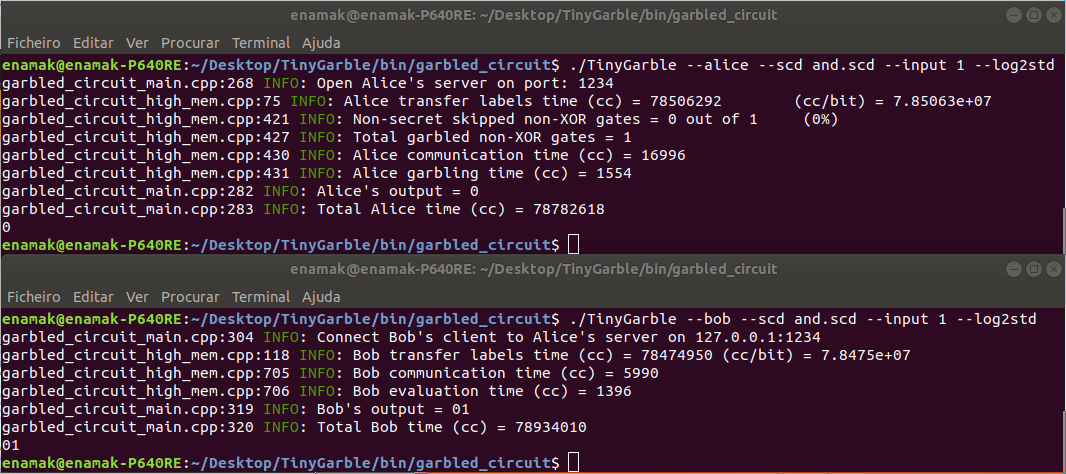
\includegraphics[width=1\textwidth, height=3.8cm]{./sdf/tiny_garble/figures/tinygarble_and_a.png}
    \caption{"And" function executed by Alice and Bob, with inputs 1 and 1, respectively.}\label{fig:tinygarble_and_a}
\end{figure}

\begin{figure}[H]
	\centering
	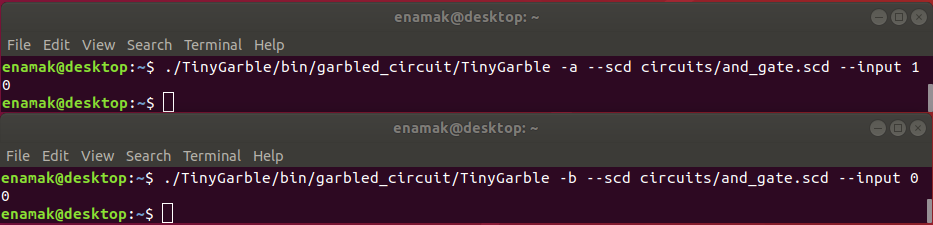
\includegraphics[width=1\textwidth, height=3.8cm]{./sdf/tiny_garble/figures/tinygarble_and_b.png}
    \caption{"And" function executed by Alice and Bob, with inputs 1 and 0, respectively.}\label{fig:tinygarble_and_b}
\end{figure}

The option 'output\_mask' allows to choose if the output will appear on Alice or Bob, 0 and 1, respectively, beeing the default value 0.

\begin{figure}[H]
	\centering
	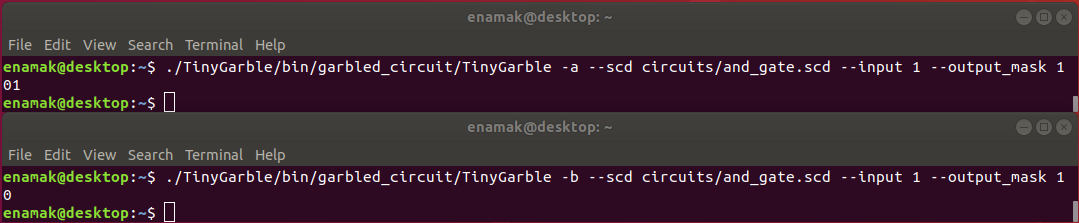
\includegraphics[width=1\textwidth, height=3.8cm]{./sdf/tiny_garble/figures/tinygarble_and_c.png}
    \caption{"And" function executed by Alice and Bob, with inputs 1 and 1, respectively. Example of output\_mask option.}\label{fig:tinygarble_and_c}
\end{figure}

\newpage

By default the information about the computation is stored in a log file, in the same folder where the TinyGarble executable is located (also works for the V2SCD\_Main and SCD\_Evaluator\_Main programs) . The option 'log2std' allows to print the information in the terminal instead of creating the log file.

\begin{figure}[H]
	\centering
	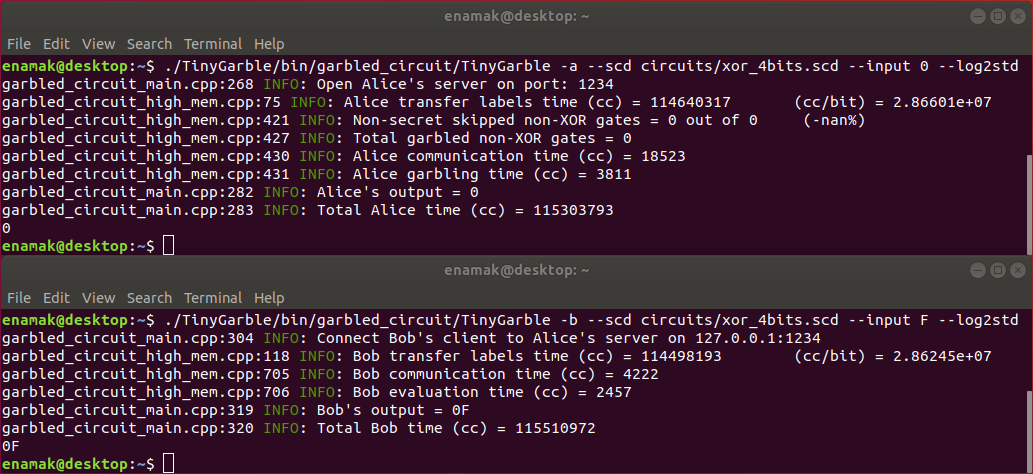
\includegraphics[width=1\textwidth, height=6.25cm]{./sdf/tiny_garble/figures/tinygarble_xor_4bits.png}
    \caption{"Xor" function with 4 bits executed by Alice and Bob, with inputs 0 and F, respectively. Example of option 'log2std'.}\label{fig:tinygarble_xor}
\end{figure}

\subsubsection{Using VHDL}

If the desirable input is VHDL, this next tool, V2VHDL, will be necessary to translate it into Verilog, which is the input supported by the RTL Synthesis Tool mentioned before.
Before cloning vhd2vl at \url{https://github.com/ldoolitt/vhd2vl} and building it, some dependencies have to be installed:

\begin{lstlisting}[caption={Installation of VHD2VL}, language=bash, captionpos=b]
$ sudo apt install flex
$ sudo apt install bison
$ git clone https://github.com/ldoolitt/vhd2vl
$ cd vhd2vl/src
$ make
$ sudo cp vhd2vl /usr/local/bin
\end{lstlisting}

To use it simply run:

\begin{lstlisting}[caption={Translation of VHDL file into Verilog}, language=bash, captionpos=b]
$ vhd2vl and_gate.vhd and_gate.v	
\end{lstlisting}

\newpage

\subsection{Programming}

\subsubsection{Folder Layout}

\begin{enumerate}
\item a23: Low level functions wrote in C.
\item bin: Created when building TinyGarble. Holds executables and examples of netlist and scd files.
\item circuit\_synthesis: Holds netlist and RTL Verilog files and the custom libs to use with Yosys. Examples below.
\item crypto: Holds C++ files for the Oblivious Transfer and their data structure, 'block'.
\item garbled\_circuit: Holds C++ files to deal with the garbling and evaluation of a circuit.
\item scd:  Holds C++ files of the SCD Converter and Evaluator mentioned before, and of the netlist Parser.
\item tcpip: Holds C++ files that deal with server connection.
\item util: Holds C++ support files.
\end{enumerate}

This subsection will show an example of a function described in a sequential circuit, more specifically the sum function located at TinyGarble/circuit\_synthesis/sum. For this example the CC parameter was set to the same as N, otherwise if kept at 1 it would be a combinational circuit. If CC is set to the same as N, each clock cycle will read one bit from the input, and also output 1 bit. So in this case if the 'clock\_cycle' option of TinyGarble is set to 8, it would read 8 bits total from 'g\_input' and 'e\_input', and would write 8 bits to 'o'. If CC was set to 2 for example, each cycle would read and write N/2 bits, if set to N/2, each cycle would read and write 2 bits. If the input given is smaller than expected size, it will be read as 0 on the clock cycles were the input is non existent.

After doing the steps explained at 'Using' section, (with the respective names for the files), the sum.scd file can be be executed as showed before with the and\_gate.scd.

When working with sequential circuits, we may want the output of each clock to be printed concatenated, separated (starting from the smallest bit), or print only the last clock output, and for that the option 'output\_mode' can be used, with values 0, 1 and 2, respectively, beeing the default 0 (it also works with SCD\_Evaluator\_Main program). The output is printed in hexadecimal format.

\begin{figure}[H]
	\centering
	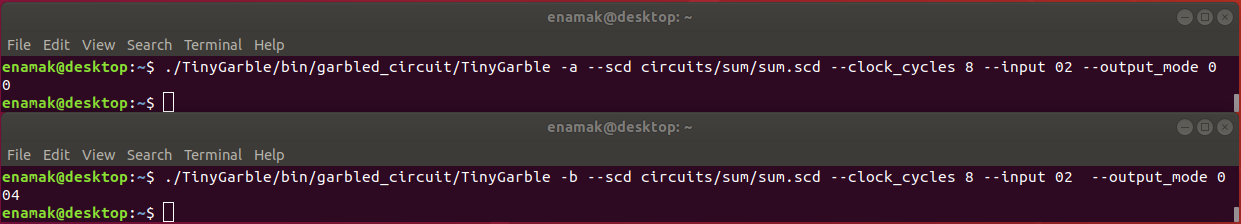
\includegraphics[width=1\textwidth, height=4cm]{./sdf/tiny_garble/figures/tinygarble_sum_0.png}
    \caption{"Sum" function with 8 bits/clocks executed by Alice and Bob, with inputs 02 and 02, respectively. Printing output concatenated(8 bits).}\label{fig:tinygarble_sum_0}
\end{figure}

\begin{figure}[H]
	\centering
	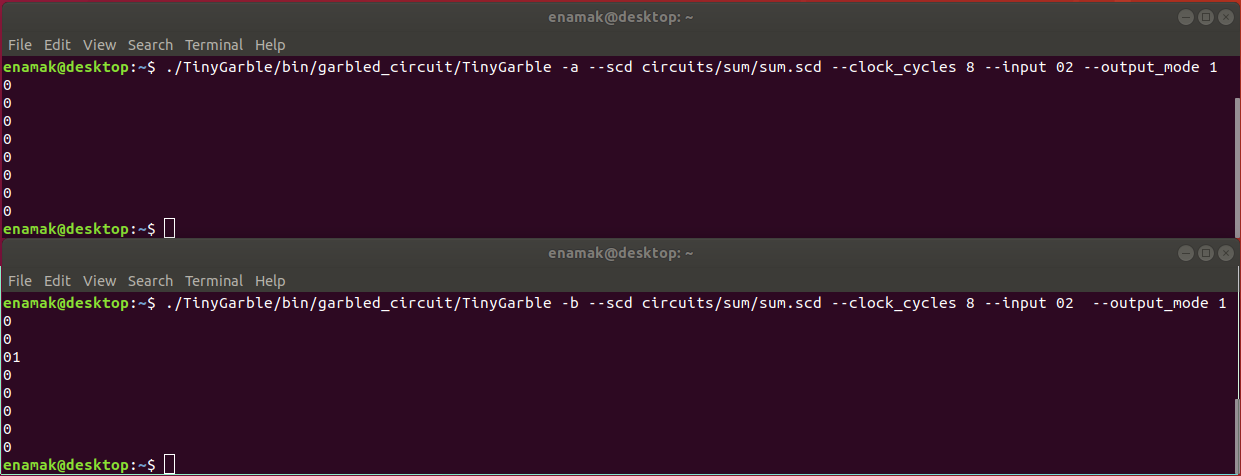
\includegraphics[width=1\textwidth, height=7cm]{./sdf/tiny_garble/figures/tinygarble_sum_1.png}
    \caption{"Sum" function with 8 bits/clocks executed by Alice and Bob, with inputs 02 and 02, respectively. Printing output separated(1 bit each cycle).}\label{fig:tinygarble_sum_1}
\end{figure}

\begin{figure}[H]
	\centering
	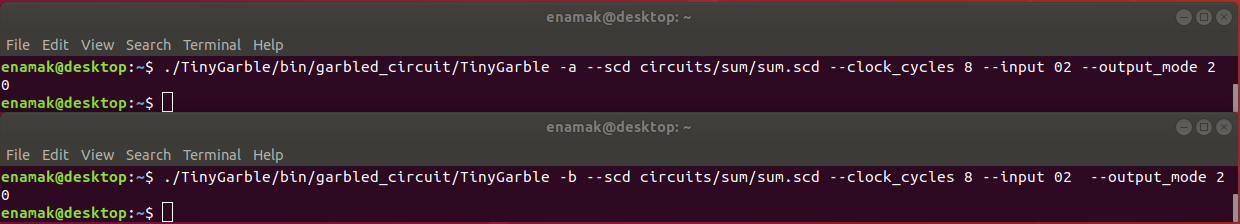
\includegraphics[width=1\textwidth, height=4cm]{./sdf/tiny_garble/figures/tinygarble_sum_2.png}
    \caption{"Sum" function with 8 bits/clocks executed by Alice and Bob, with inputs 02 and 02, respectively. Printing the last clock cycle output (last bit of output).}\label{fig:tinygarble_sum_2}
\end{figure}

\subsubsection{Running on seperate Hosts}

To run Bob and Alices in different hosts, the host running Bob has to give an extra option '-s <Alice IP adress>'. To find the ip adress run 'hostname -I' or 'ifconfig' in Alice's terminal. The default port is 1234, to change it add the optionn -p <port> on both Hosts. The example below assumes Alice's IP adress is 192.168.1.3. The '--output\_mask arg <0 or 1>' can also be used, to determine which host shows the output, the default is 0 (Bob), and can be changed to 1 (Alice).
\begin{lstlisting}[caption={Installation of Yosys-abc for Ubuntu 15.04>}, language=bash, captionpos=b]
alice@ubuntu:~$ ./TinyGarble/bin/garbled_circuit/TinyGarble -a 
-i circuits/and.scd -p 3000 --input 1
bob@ubuntu:~$ ./TinyGarble/bin/garbled_circuit/TinyGarble -b 
-i  circuits/and.scd -s 192.168.1.3 --p 3000 --input 1
\end{lstlisting}

\subsubsection{Keys}

Since TinyGarble is based on JustGarble, it's garbling scheme will be based on fixed-key AES.
Alice generates a random key, 'with the randomBlock() function', that will then be expanded 10 times (128bit AES), thus if a custom key is wanted, 128*11 bits are needed.

Below is the struct used to represent the AES\_KEY, present at TinyGarble/crypto/aes.h:

\begin{lstlisting}[caption={AES\_KEY struct}, language=C, captionpos=b]
typedef struct {
  __m128i rd_key[15];
  int rounds;
} AES_KEY;
\end{lstlisting}

The \_\_m128i variable represents a 128bit register, the rd\_key[0] holds the global\_key, and rd\_key[10:1] will have the expanded keys. rd\_key[15:11] are only used for 192 or 256 bit AES. Rounds represent the number of times the key was expanded (10, in case of 128bit AES).

The following function "AES128KeyExpansion" located at the same file, expands the 128 bit global\_key into more ten 128 bit keys, that are stored in rd\_key[10:1], as mentioned before.

\begin{lstlisting}[caption={AES Expansion function}, language=C, captionpos=b]
inline void AES128KeyExpansion(const unsigned char *userkey, void *key) {
  __m128i x0, x1, x2;
  __m128i *kp = (__m128i *) key;
  kp[0] = x0 = _mm_loadu_si128((__m128i *) userkey);
  x2 = _mm_setzero_si128();
  EXPAND_ASSIST(x0, x1, x2, x0, 255, 1);
  kp[1] = x0;
  EXPAND_ASSIST(x0, x1, x2, x0, 255, 2);
  kp[2] = x0;
  EXPAND_ASSIST(x0, x1, x2, x0, 255, 4);
  kp[3] = x0;
  EXPAND_ASSIST(x0, x1, x2, x0, 255, 8);
  kp[4] = x0;
  EXPAND_ASSIST(x0, x1, x2, x0, 255, 16);
  kp[5] = x0;
  EXPAND_ASSIST(x0, x1, x2, x0, 255, 32);
  kp[6] = x0;
  EXPAND_ASSIST(x0, x1, x2, x0, 255, 64);
  kp[7] = x0;
  EXPAND_ASSIST(x0, x1, x2, x0, 255, 128);
  kp[8] = x0;
  EXPAND_ASSIST(x0, x1, x2, x0, 255, 27);
  kp[9] = x0;
  EXPAND_ASSIST(x0, x1, x2, x0, 255, 54);
  kp[10] = x0;
}
\end{lstlisting}

To use a non AES Key, instead of giving a global key and expand it, all 11 different keys have to be provided, and stored on rd\_key[10:0].
To do that, the intrinsic function '\_mm\_loadu\_si128' can be used, as showed in the example below.

\begin{lstlisting}[caption={Storing four ints into a 128bit register. It should ouput "50607080 10203040 0fedcba9 87654321".}, language=C, captionpos=b]
  block keyBlock;
  Str2Block("50607080 10203040 0fedcba9 87654391", &keyBlock);
  __m128i teste = _mm_loadu_si128((__m128i *)((unsigned char *)&keyBlock));
  int32_t *tmpl = (int32_t *) &teste;
  printf("%.8x %.8x %.8x %.8x\n", tmp[3], tmp[2], tmp[1], tmp[0]);
\end{lstlisting}

The same process has to be repeated for the remaining 10 keys.

\subsubsection{Moda function}

The purpose of this function is to take two inputs from each host, and return 0 if the first inputs of each host summed are greater than the sum of the second inputs, and return 1 otherwise. It outputs 2 if both sums are equal.
Examples:
\begin{enumerate}
\item a: \begin{lstlisting}[caption={Example of moda inputs and output}, captionpos=b]
Alice -> 5,10   Bob -> 9, 1   Output -> 0
\end{lstlisting}
\item b: \begin{lstlisting}[caption={Example of moda inputs and output}, captionpos=b]
Alice -> 1,3   Bob -> 6, 9   Output -> 1
\end{lstlisting}
\end{enumerate}

This function can be both implemented with a combinational and sequential circuit, although with the combinational the maximum size of the inputs has to be set, and cannot be changed between executions.
The module 'ADD', which represents a full adder, located at 'TinyGarble/circuit\_synthesis/syn\_lib' (folder mentioned before) was used, so the command read\_verilog TinyGarble/circuit\_synthesis/syn\_lib/*.v has to be used.

The following verilog module shows the combinationl circuit:

\newpage

\begin{lstlisting}[caption={moda.v}, language=Verilog, captionpos=b]
module moda(g_input, e_input, o);

	input[31:0] g_input, e_input;
	wire[16:0] tmp_0, tmp_1;
	output [1:0] o;

	ADD 
	#(
		.N(16)
	)
	input_0
	(
		.A(g_input[31:16]),
		.B(e_input[31:16]),
		.CI(),
		.S(tmp_0[15:0]),
		.CO(tmp_0[16:16])
	);
	ADD 
	#(
		.N(16)
	)
	input_1
	(
		.A(g_input[15:0]),
		.B(e_input[15:0]),
		.CI(),
		.S(tmp_1[15:0]),
		.CO(tmp_1[16:16])
	);	

	always@ *
	begin
		if(tmp_0 > tmp_1)
			o <= 0;
		else if(tmp_0 < tmp_1)
			o <= 1;
		else
			o <= 2;
	end
endmodule
\end{lstlisting}

\newpage
Since the garblers and evaluator inputs have 32 bits, values between 0 and 9999 are accepted. The sums will be made in hexadecimal even if the input is intented to be decimal, but the output should not be affected.

Examples:

\begin{figure}[H]
	\centering
	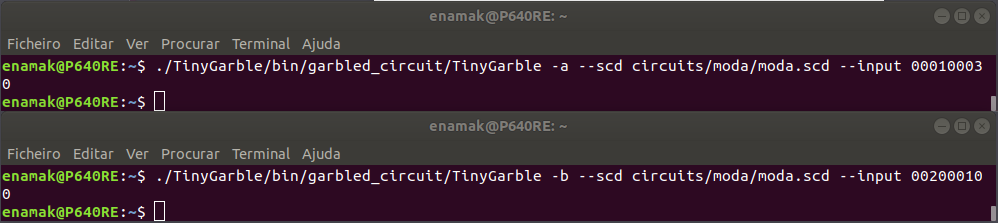
\includegraphics[width=1\textwidth, height=3.8cm]{./sdf/tiny_garble/figures/tinygarble_moda_0.png}
    \caption{"Moda" function executed by Alice and Bob, with inputs 00010003(1,3) and 00200010(20,10), respectively.}\label{fig:tinygarble_moda_0}
\end{figure}

\begin{figure}[H]
	\centering
	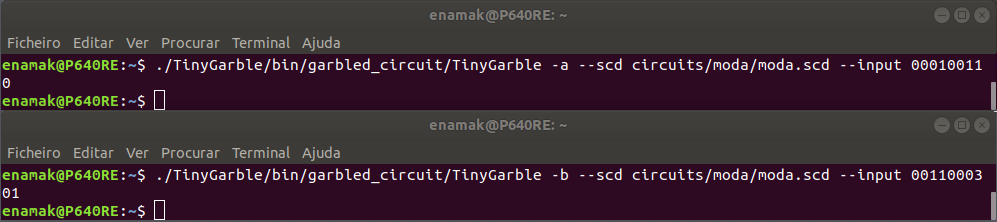
\includegraphics[width=1\textwidth, height=3.8cm]{./sdf/tiny_garble/figures/tinygarble_moda_1.png}
    \caption{"Moda" function executed by Alice and Bob, with inputs 00010011(1,11) and 00110003(11,3), respectively.}\label{fig:tinygarble_moda_1}
\end{figure}

\begin{figure}[H]
	\centering
	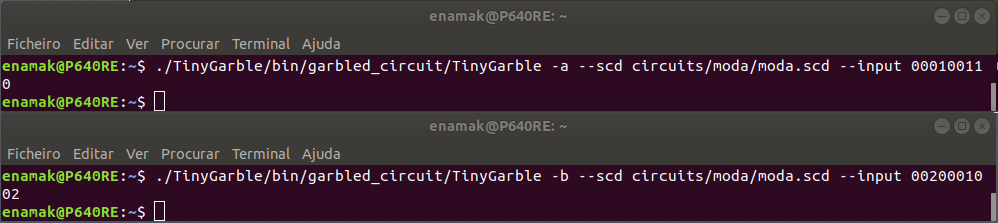
\includegraphics[width=1\textwidth, height=3.8cm]{./sdf/tiny_garble/figures/tinygarble_moda_2.png}
    \caption{"Moda" function executed by Alice and Bob, with inputs 00010011(1,11) and 00200010(20,10), respectively.}\label{fig:tinygarble_moda_2}
\end{figure}

\newpage
\subsubsection{TinyGarble Interface}

To ease the computation of the moda function between Alice and Bob, the interface 'STPC' was made. It can be found at sdf/tiny\_garble/STPC zip, which containts a folder with the src files, and the folder with the built project. The interface was made with QTCreator, which contains the libraries required for the interface and sockets, so in case any changes have to be made to the interface itself or to the c++ files, it has to be installed. QTCreator 5.11.3 was used, and installed with the '.run' file downloaded at QT's website.
After opening the project with the '.pro' file located at the work folder, this one and the build folder can be configured in 'Projects', which are in this case STCP-src and STPC-gui, respectively.

In order to make the app usable in any linux system, \url{https://github.com/probonopd/linuxdeployqt} was used, more specifically the linuxdeployqt-5-x86\_64.AppImage file, that can be found at the Git's Releases tab. It essentialy creates a bundle with all the libraries and other necessary files to execute the app.

\begin{lstlisting}[caption={Deploying QT application. Executable in this case is at STPC-gui/STPC}, language=bash, captionpos=b]
$ export PATH=/[pathToQt]/[version]/gcc/bin:$PATH
$ chmod a+x linuxdeployqt-5-x86_64.AppImage-x86_64.AppImage
$ ./linuxdeployqt-5-x86_64.AppImage-x86_64.AppImage [PathToExecutable]
\end{lstlisting}

If no error ocurred, one should be able to go to the folder where the built project is, and run the executable, in this case './STPC'.
When opening the interface, the user has to insert the path to TinyGarble, and the path to the folder containing the 'moda.scd' file, before choosing which host he will be (Alice or Bob).

\begin{figure}[H]
	\centering
	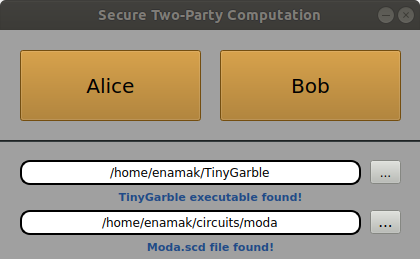
\includegraphics[width=.8\textwidth, height=6cm]{./sdf/tiny_garble/figures/STPC_start.png}
    \caption{Starting window of STPC interface.}\label{fig:STPC_start}
\end{figure}

If Alice was selected, the user will have to insert the PORT for TinyGarble's connection, and the IP Adress of the Key provider and the respective PORT for the connection.

\begin{figure}[H]
	\centering
	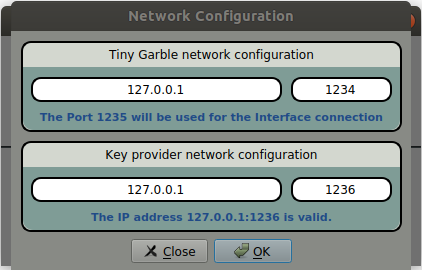
\includegraphics[width=.8\textwidth, height=6cm]{./sdf/tiny_garble/figures/STPC_alice.png}
    \caption{Alice network configuration.}\label{fig:STPC_alice}
\end{figure}

For Bob, only the IP Adress of Alice and the respective PORT are needed.

\begin{figure}[H]
	\centering
	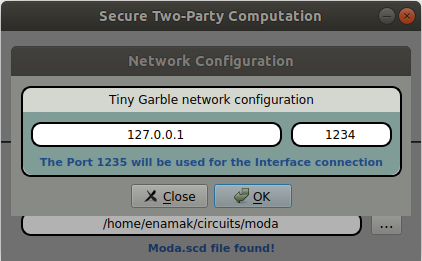
\includegraphics[width=.8\textwidth, height=6cm]{./sdf/tiny_garble/figures/STPC_bob.png}
    \caption{Bob network configuration.}\label{fig:STPC_bob}
\end{figure}

After all configuration is done, the final window will appear. In this window the user can request the computation of the moda function, or accept it in case the other party requested it first.
The blue frame shows warnings and information about the connection and current state of the application.

\begin{figure}[H]
	\centering
	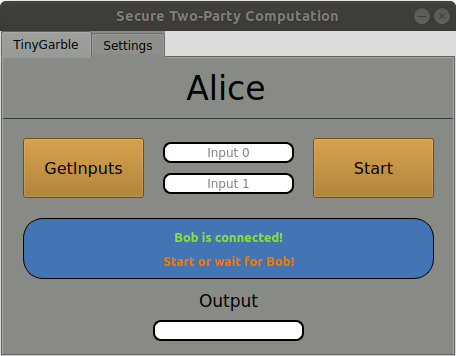
\includegraphics[width=.8\textwidth, height=6cm]{./sdf/tiny_garble/figures/STPC_a.png}
    \caption{STPC main window.}\label{fig:STPC_a}
\end{figure}

\subsubsection{Server to provide Keys}

This next program, 'key\_server', is a TCP server that provides a random number in binary with N bits, when receiving an 'N' from a client. It will respond with a error message if N is not a number.
It is used in the Interface showed above, to retrieve the Key for Alice. Each time a computation is accepted by any of the hosts, Alice will connect to the key provider, send a message 'N', and receive the random number that can then be used as the Key to generate the Garbled Circuit.
Qt network libraries were used, so Qt will need to be installed, and the app can be built and deployed the same way the interface app is.

\begin{lstlisting}[caption={Deploying QT application}, language=bash, captionpos=b]
$ ./key_server [pathToKeysTxt] [PORT]
\end{lstlisting}

\subsection{Open Issues}

\begin{enumerate}  
\item No free High Level Synthesis was yet found, so impossible to run examples with C or C++ as input.
\end{enumerate}

% bibliographic references for the section ----------------------------
\clearpage
\printbibliography[heading=subbibliography]
\end{refsection}
\addcontentsline{toc}{subsection}{Bibliography}
\cleardoublepage
% --------------------------------------------------------------------
